\documentclass[12pt]{amsproc}

% a la fullpage
\usepackage{geometry}
\geometry{a4paper}
\geometry{twoside=false}

% Activate to begin paragraphs with an empty line rather than an indent
\usepackage[parfill]{parskip}
\setlength{\marginparwidth}{2cm}

\newtheorem{theorem}{Theorem}[section]
\newtheorem{definition}[theorem]{Definition}
\newtheorem{lemma}[theorem]{Lemma}

\usepackage{graphicx}
\usepackage{float}
\usepackage{amssymb}
\usepackage{color}
\usepackage{listings}

\newcommand{\id}{\text{id}}
\newcommand{\N}{\mathbb{N}}
\newcommand{\Z}{\mathbb{Z}}
\newcommand{\R}{\mathbb{R}}
\newcommand{\cat}[1]{\mathbf{#1}}
\newcommand{\Ch}[1]{\mathbf{Ch}(#1)}
\newcommand{\Hom}[3]{\mathbf{Hom}_{#1}(#2, #3)}

\newcommand{\iso}{\cong}
\newcommand{\tot}[1]{\xrightarrow{\,\,{#1}\,\,}}
\newcommand{\eps}{\varepsilon}
\newcommand{\I}{\,\mid\,}
\newcommand{\then}{\Rightarrow}
\newcommand{\inject}{\hookrightarrow}
\newcommand{\del}{\partial}
\newcommand{\nsubgrp}{\trianglelefteq}

% relative to the one who includes us :(
\graphicspath{ {../images/} }

\newcommand{\todo}[1]{
	\addcontentsline{tdo}{todo}{\protect{#1}}
	$\ast$ \marginpar{\tiny $\ast$ #1}
}
\makeatletter
	\newcommand \listoftodos{\section*{Todo list} \@starttoc{tdo}}
	\newcommand\l@todo[2]{
		\par\noindent \textit{#2}, \parbox{10cm}{#1}\par
	}
\makeatother


\title{Dold-Kan Correspondence}
\author{Joshua Moerman}

\begin{document}
\maketitle

\section*{Introduction}
In this thesis we will look at a correspondence which was discovered by A. Dold and D. Kan independently, hence it is called the \emph{Dold-Kan correspondence}. Abstractly it is the following equivalence of categories:
$$ \Ch{\Ab} \simeq \sAb $$
It is interesting because objects on the left hand side are considered to be algebraic of nature, whereas objects on the right are more topological. In particular this correspondence also gives a isomorphism between homology groups (on the left hand side) and homotopy groups (on the right hand side). A bit more precise:
$$ \pi_n(A) \iso H_n(N(A)) \text{ for all } n \in \N $$
where $N: \sAb \to \Ch{\Ab}$ is one half of the equivalence.

\newpage
\section{Category Theory}
\label{sec:Category Theory}
Before we will introduce the two categories $\Ch{\Ab}$ and $\sAb$, we will first look at some basic category theory. If one is already familier with these concepts, he or she can skip this section. We will introduce the notions of categories, functors, isomorphims, natural transformations, equivalences (between categories) and adjunctions.

\subsection{Categories}
\begin{definition}
	A \emph{category} $\cat{C}$ consists of a collection \emph{objects}, and for each two objects $A$ and $B$ in $\cat{C}$ there is a (possibly empty) \emph{set of maps} (or arrows) from $A$ to $B$, notated as $\Hom{\cat{C}}{A}{B}$, such that:
	\begin{itemize}
		\item \emph{(Identity)}
			$\id_A \in \Hom{\cat{C}}{A}{A}$ for all $A$ in $\cat{C}$,
		\item \emph{(Composition)}
			for any $f \in \Hom{\cat{C}}{A}{B}$ and $g \in \Hom{\cat{C}}{B}{C}$ we have $g \circ f \in \Hom{\cat{C}}{A}{C}$,
		\item \emph{(Associativity)}
			$f \circ (g \circ h) = (f \circ g) \circ h$, and
		\item \emph{(Identity law)}
			$\id_B \circ f = f = f \circ \id_A$ for all $f \in \Hom{\cat{C}}{A}{B}$.
	\end{itemize}
\end{definition}

Note that the collection of objects may be a proper class instead of a set, however we will notate $A \in \cat{C}$ if $A$ is an object of $\cat{C}$. And instead of writing $f \in \Hom{\cat{C}}{A}{B}$, we write $f: A \to B$.

As the notation suggests maps can be thought of as functions, which is also the case in many examples.

\begin{example}
	The category $\Set$ has a objects sets, and as maps ordinary functions. Of course we then have the identity function $\id_X(x) = x$ and composition as usual.
\end{example}
\begin{example}
	The category $\Ab$ has a objects abelian groups, and the maps between two objects are exactly the grouphomomorphisms. We know that the identity function is indeed a grouphomomorphism, and composing two grouphomomorpisms, gives indeed a new grouphomomorphism.
\end{example}

In fact almost any mathematical structure can be described as a category, we have: $\cat{Ring}$ for rings, $\cat{Vect}$ for $\R$-vectorspaces, $\cat{Set_{fin}}$ for finite sets, $\cat{Poset}$ for posets, etc. Of course we would also like to express relations between categories, for example every abelian group is also a set. This idea can be formulated by the notion of a functor.

\begin{definition}
	A \emph{functor} $F$ between a category $\cat{C}$ and $\cat{D}$ consists of a function $F_0$ from the objects of $\cat{C}$ to the objects of $\cat{D}$ and a function $F_1$ from maps in $\cat{C}$ to maps in $\cat{D}$, such that:
	\begin{itemize}
		\item for $f: A \to B$, we have $F_1(f): F_0(A) \to F_0(B)$,
		\item $F_1(\id_A) = \id_{F_0(A)}$ and
		\item $F_1(f \circ g) = F_1(f) \circ F_1(g)$.
	\end{itemize}
	We normally do not write the index of $F_0$ or $F_1$, instead we wrtie $F$ for both functions.
\end{definition}
\todo{CT: contravariant functor}

\begin{exlemma}
	There is a category $\cat{Cat}$ with categories as objects, and functors as maps.
\end{exlemma}
\begin{proof}
	First we define the identity functor. Let $\cat{C}$ be a category, define $\id_\cat{C}(A) = A$ for any object $A \in \cat{C}$ and $\id_\cat{C}(f) = f$ for any map $f: A \to B$ in $\cat{C}$. Cleary we have $\id_\cat{C}(f) : \id_\cat{C}(A) \to \id_\cat{C}(B)$. Also $\id_\cat{C}(\id_A) = \id_A = \id_{\id_\cat{C}(A)}$ and $\id_\cat{C}(f \circ g) = f \circ g$. So indeed $\id_\cat{C}$ is a functor.

	Given a functors $F: \cat{C} \to \cat{D}$ and $G: \cat{D} \to \cat{E}$, we can define the composition $G \circ F$ on objects as $G \circ F(A) = G(F(A))$ and on maps as $G \circ F(f) = G(F(f))$. This again is a functor $G \circ F$, we will not spell out the details.

	The remaining requirements are the associativity and identity law. We also leave these to the reader.
\end{proof}

\subsection{Isomorphisms}
Given a category $\cat{C}$ and two objects $A, B \in \cat{C}$ we would like to know when those objects are regarded as the same, according to the category. This will be the case when there is an isomorphism between the two.

\begin{definition}
	A map $f: A \to B$ in a category $\cat{C}$ is an isomorphism if there is a map $g: B \to A$ such that:
	$$ f \circ g = \id_B \text{ and } g \circ f = id_A.$$
\end{definition}

Isomorphisms in $\Ab$ are exactly the isomorphisms which we know, ie. the grouphomomorphisms which are both injective and surjective.
For example the cyclic group $\Z_4$ and the klein four-group $V_4$ are not isomorphic in $\Ab$, but if we regard only the sets $\Z_4$ and $V_4$, then they are (because there is a bijection). So it is good to note that whether two objects are isomorphic  really depends on the category we are working in.

\todo{CT: Equivalence / natro}
\todo{CT: Adjunction}
\todo{CT: Yoneda?}

\newpage
\section{Chain Complexes}
\label{sec:Chain Complexes}
\begin{definition}
	A chain complex $C$ is a collection of abelian groups $C_n$ together with boundary operators $\del_n: C_{n+1} \to C_n$, such that $\del_n \circ \del_{n+1} = 0$. The collections of all such objects will be denoted by $\Ch{\cat{Ab}}$.
\end{definition}

In other words a chain complex is the following diagram.
$$ \cdots \to C_4 \to C_3 \to C_2 \to C_1 \to C_0 $$

Of course we can make this more general by taking for example $R$-modules instead of abelian groups. We will later see which kind of algebraic objects make sense to use in this definition. The boundary operators give rise to certain subgroups, because all groups are abelian, subgroups are normal subgroups.

\begin{definition}
	Given a chain complex $C$ we define the following subgroups:
	\begin{itemize}
		\item $Z_n(C) = ker(\del: C_n \to C_{n-1}) \nsubgrp C_n$, and
		\item $B_n(C) = im(\del: C_{n+1} \to C_n) \nsubgrp C_n$.
	\end{itemize}
\end{definition}
\begin{lemma}
	Given a chain complex $C$ we have for all $n \in \N$:
	$$ B_n(C) \nsubgrp Z_n(C).$$
\end{lemma}
\begin{proof}
	It follows from $\del_n \circ \del_{n+1} = 0$ that $im(\del: C_{n+1} \to C_n)$ is a subset of $ker(\del: C_n \to C_{n-1})$. Those are exactly the abelian groups $B_n(C)$ and $Z_n(C)$, so $ B_n(C) \nsubgrp Z_n(C) $.
\end{proof}
\begin{definition}
	Given a chain complex $C$ we define the \emph{$n$-th homology group} $H_n(C)$:
	$$ H_n(C) = Z_n(C) / B_n(C).$$
\end{definition}

\subsection{The singular chain complex}
In order to see why we are interested in the construction of homology groups, we will look at an example from algebraic topology. We will see that homology gives a nice invariant for spaces. So we will form a chain complex from a topological space $X$. In order to do so, we first need some more notions.
\begin{definition}
	The topological space $\Delta^n$ is called the \emph{topological $n$-simplex} and is defined as:
	$$ \Delta^n = \{x \in \R^{n+1} \I x_i \geq 0 \text{ and } x_0 + \ldots + x_n = 1 \}.$$
	The topology on $\Delta^n$ is the subspace topology.
\end{definition}

In particular $\Delta^0$ is simply a point, $\Delta^1$ a line and $\Delta^2$ a triangle. There are nice inclusions $\Delta^n \mono \Delta^{n+1}$ which we need later on. For any $n \in \N$ we define:
\begin{definition}
	For $i \in \{0, \ldots, n+1\}$ the $i$-th face map $\delta^i : \Delta^n \mono \Delta^{n+1}$ is defined as:
	$$ \delta^i (x_0, \ldots, x_n) = (x_0, \ldots, x_{i-1}, 0, x_{i+1}, \ldots, x_n) \text{ for all } x \in \Delta^n.$$
\end{definition}

Note that if we have any continuous map $\sigma : \Delta^{n+1} \to X$ we can precompose with a face map to get $\sigma \circ \delta^i : \Delta^n \to X$. This will be used for defining the boundary operator. We can make pictures of this, and when concerning continuous maps $\sigma : \Delta^{n+1} \to X$ we will draw the images in the space $X$, instead of functions.

\todo{Ch: Make some pictures here}

\todo{Ch: Define free abelian group}

We now have enough tools to define the singular chain complex of a space $X$.

\begin{definition}
	For a topological space $X$ we define an abelian group $C_n(X)$ as follows.
	$$ C_n(X) = \Z[\Hom{\cat{Top}}{\Delta^n}{X}] $$
	The boundary operator $\del : C_{n+1}(X) \to C_n(X)$ is defined on generators as:
	$$ \del(\sigma) = \sigma \circ \delta^0 - \sigma \circ \delta^1 + \ldots + (-1)^{n+1} \sigma \circ \delta^{n+1}.$$
\end{definition}

This might seem a bit complicated, but we can pictures this in an intuitive way, as in figure~\ref{fig:singular_chaincomplex3}. And we see that the boundary operators really give the boundary of an $n$-simplex. To see that this indeed is a chain complex we have to proof that the composition of two such operators is the zero map.
\begin{figure}
	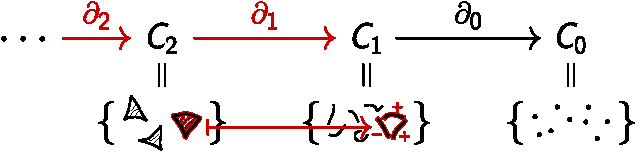
\includegraphics{singular_chaincomplex3}
	\caption{The boundary of a 2-simplex}
	\label{fig:singular_chaincomplex3}
\end{figure}

\todo{Ch: Proposition: $C(X) \in \Ch{\cat{Ab}}$}

\todo{Ch: Example homology of some space}

\todo{Ch: Show that $\Ch{\Ab}$ is an ab. cat. At least show functoriality $\Hom{\Ch{\Ab}}{-}{-}$}


\newpage
\listoftodos
% \nocite{*}
% \bibliographystyle{alpha}
% \bibliography{references}	
\end{document}
